\section{Sorting}
Sorting elements in an array $A[1 \ldots n]$,
is usually a \emph{Fundamental Task}, often first step in analysis.
How do we sort?
Let's begin with solving simpler problem.

\AlgoInput Given 2 sorted arrays, $B[1 \ldots n]$ and $C[1 \ldots m]$.

\AlgoOutput Combine two arrays into sorted $A[1 \ldots n+m]$.

\solution

Keep a pointer to each array starting at first element,
compare values at pointers, take smaller and advance pointers.
The algorithm is described in \cref{algo:merge}.

\begin{algorithm}[H]
    \caption{Merge Two Sorted Arrays}\label{algo:merge}
    \begin{algorithmic}[1]
        \Procedure{Merge}{$A[1 \ldots n+m], B[1 \ldots n], C[1 \ldots m]$}
            \State $Bindex = 1$, $Cindex = 1$
            \For{$Aindex = 1 \text{ to } n+m$}
                \If{$Cindex > m$}\Comment{$C$ exhausted.}
                    \State $A[Aindex] = B[Bindex]$
                    \State $Bindex++$
                \ElsIf{$Bindex > n$}\Comment{$B$ exhausted.}
                    \State $A[Aindex] = C[Cindex]$
                    \State $Cindex++$
                \ElsIf{$B[Bindex] < C[Cindex]$}\Comment{$B$ smaller.}
                    \State $A[Aindex] = B[Bindex]$
                    \State $Bindex++$
                \Else \Comment{$C$ smaller.}
                    \State $A[Aindex] = C[Cindex]$
                    \State $Cindex++$
                \EndIf
            \EndFor
        \EndProcedure
    \end{algorithmic}
\end{algorithm}

Merging takes \bigO{n+m} time.

\subsection{Insertion Sort \& Merge Sort}
Given a bag of $n$ items (e.g playing cards).
\begin{enumerate}
    \item Pick up one item at a time.
    \item Put item into sorted set of previous items.
\end{enumerate}
The algorithm is described in \cref{algo:insertion}.

\begin{algorithm}[H]
    \caption{Insertion Sort}\label{algo:insertion}
    \begin{algorithmic}[1]
        \Procedure{InsertionSort}{$A[1 \ldots n]$}
            \For{$j = 2 \text{ to } n$}
                \State $key = A[j]$
                \State $i = j - 1$
                \While{$i > 0 \text{ and } A[i] > key$}
                    \State $A[i+1] = A[i]$
                    \State $i = i - 1$
                \EndWhile
                \State $A[i+1] = key$
            \EndFor
        \EndProcedure
    \end{algorithmic}
\end{algorithm}

Loop invariant: at start of each loop iteration,
$A[1 \ldots n]$ consists of original $A[1 \ldots j-1]$ elements,
but in sorted order.

Thus, we can rewrite insertion sort using \ProcedureName{Merge}{}
as shown in \cref{algo:ris}.

\begin{algorithm}[H]
    \caption{Combine Insertion Sort with Merge}\label{algo:ris}
    \begin{algorithmic}[1]
        \Procedure{IS}{$A[1 \ldots n]$}
            \For{$j = 2 \text{ to } n$}
                \State\ProcedureName{Merge}{A[1 \ldots j], A[1 \ldots j-1], A[j]}
            \EndFor
        \EndProcedure
        \Procedure{RIS}{$A[1 \ldots n]$} \Comment{Recursive Rewrite.}
            \If{$n>1$}
                \State\ProcedureName{RIS}{A[1 \ldots n-1]}
                \State\ProcedureName{Merge}{A[1 \ldots n], A[1 \ldots n-1], A[n]}
            \EndIf
        \EndProcedure
    \end{algorithmic}
\end{algorithm}

How long does RIS takes?
$T(n) = T(n-1) + \Theta(n) = \Theta(n^2)$.

Can we do better? Yes! Divide and Conquer, cut in the middle,
which leads to merge sort as described in \cref{algo:mergesort}.

\begin{algorithm}[H]
    \caption{Merge Sort}\label{algo:mergesort}
    \begin{algorithmic}[1]
        \Procedure{MergeSort}{$A[1 \ldots n]$}
            \If{$n>1$}
                \State\ProcedureName{MergeSort}{A[1 \ldots \lfloor n/2 \rfloor]}
                \State\ProcedureName{MergeSort}{A[\lfloor n/2 \rfloor + 1 \ldots n]}
                \State\ProcedureName{Merge}{A[1 \ldots n], A[1 \ldots \lfloor n/2 \rfloor], A[\lfloor n/2 \rfloor +1 \ldots n]}
            \EndIf
        \EndProcedure
    \end{algorithmic}
\end{algorithm}

How long does Merge Sort takes?
$T(n) = 2T(n/2) + \Theta(n) = \Theta(n \log n)$.

\subsection{Sorting Lower Bound}
Given $A[1 \ldots n]$, assume elements distinct.
Algorithms we've seen so far sort only by comparisons,
i.e given $A[i]$ and $A[j]$, is $A[i] < A[j]$ or $A[i] > A[j]$.
How fast can comparison based sorting be?

Assume algorithms is deterministic: for any $n$ size input,
the first comparison is fixed.
The comparison tree can be described as \cref{fig:sortinglowerbound}

\begin{figure}[H]
    \caption{Comparison Tree}\label{fig:sortinglowerbound}
    \centering
    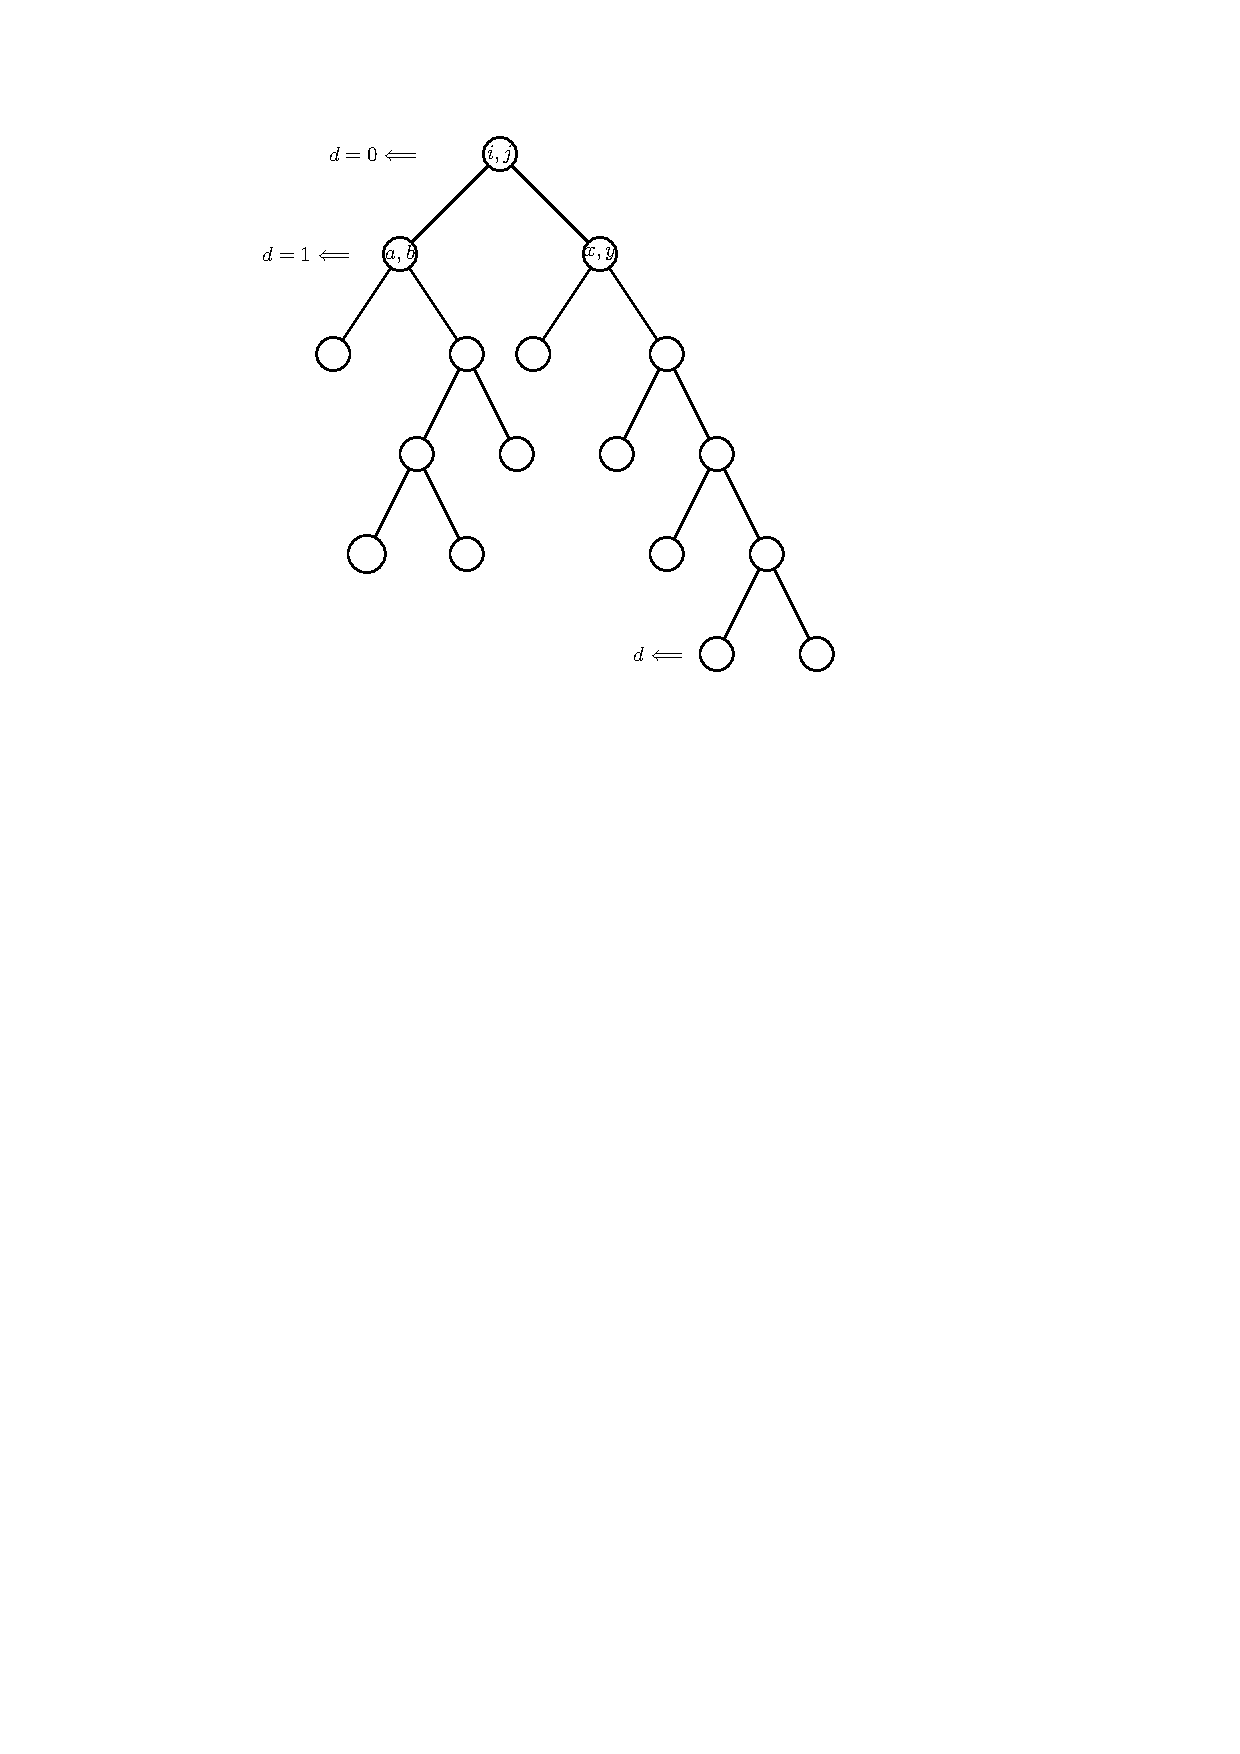
\includegraphics[scale=1.1]{fig/sortlowerbound}
\end{figure}

Meaning of the comparison tree:
\begin{itemize}
    \item Pair in node is indices of elements comparing.
    \item Left branch means $A[i] < A[j]$.
    \item Right branch means $A[i] > A[j]$.
    \item Result of comparison uniquely determines next comparison.
    \item Algorithm always terminates when tree has finite depth $d$.
    \item At leaf we determined sorted order.
    \item Depth of leafs is number of comparisons needed.
    \item worst cast = deepest leaf depth.
    \item for binary trees, number of leaves $\leq 2^d$.
\end{itemize}
In total $n!$ (factorial) ordering of elements.
\[n! \leq \text{ number of leaves } \leq 2^d\]
which means:
\[d \geq \lg(n!) = \Theta(n \log n)\]
using Stirling's Approximation $\displaystyle n! \approx \sqrt{2n}\left(\frac{n}{e}\right)^n$.

\subsection{Sorting in Linear Time}
What if allow operations other than comparisons,
and make input assumptions.

\subsubsection{Counting Sort}
Given array $A[1 \ldots n]$ of integers s.t $1 \leq A[i] \leq k$.
If $k = \bigO{n}$, then can sort in linear time. (No comparisons)

\subsubsection{Radix Sort}
Given array $A[1 \ldots n]$, assume $b$-bit integers, where $b$ is fixed value.
Sorting based on most significant bit.

\begin{algorithm}[H]
    \caption{Least Significant Radix Sort}\label{algo:lrs}
    \begin{algorithmic}[1]
        \Procedure{LRS}{$A,b$}
            \For{$i = 1 \text{ to } b$}
                \State Stable sort $A$ based on bit $i$\Comment{Stable is important!}
            \EndFor
        \EndProcedure
    \end{algorithmic}
\end{algorithm}

\subsection{Quick Sort \& Median Selection}
Quick sort is a comparison based, recursive, in place sorting (unlike radix).
Recall the \emph{Merge Sort}, using divide and conquer,
each time break in half, sort each half recursively, then combine.
Combining took $\Theta(n)$ time, $T(n) = 2T(n/2) + \Theta(n) = \Theta(n \log n)$.

Quick sort reverses the order:
\begin{quote}
    spend time to carefully split elements before recursive calls.
\end{quote}

\subsubsection{Pivoting}
Pick element $A[p]$, divide $A$ into elements smaller or larger than $A[p]$.
After pivoting, if we sort the ``$<$'' set and ``$>$'' set recursively,
we are done when recursive calls return.
The algorithm is described in \cref{algo:qs}

\begin{algorithm}[H]
    \caption{Pivoting \& Quick Sort}\label{algo:qs}
    \begin{algorithmic}[1]
        \Procedure{Pivot}{$A[1 \ldots n], p$}
            \State\ProcedureName{Swap}{A[p], A[n]}
            \State $i = 0$
            \State $j = n$
            \While{$i < j$}
                \Repeat
                    \State $i = i+1$
                \Until{$i \geq j \text{ or } A[i] \geq A[n]$}
                \Repeat
                    \State $j = j-1$
                \Until{$i \geq j \text{ or } A[j] \leq A[n]$}
                \If{$i < j$}
                    \State\ProcedureName{Swap}{A[i], A[j]}
                \EndIf
            \EndWhile
            \State\ProcedureName{Swap}{A[i], A[n]}
            \Return $i$
        \EndProcedure
        \Procedure{QuickSort}{}
            \If{$n > 1$}
                \State Choose pivot $p$
                \State $r = \ProcedureName{Pivot}{A[1 \ldots n], p}$
                \State \ProcedureName{QuickSort}{A[1 \ldots r-1]}
                \State \ProcedureName{QuickSort}{A[r-1 \ldots n]}
            \EndIf
        \EndProcedure
    \end{algorithmic}
\end{algorithm}

\analysis
Running time: pivot operation takes linear time ($\Theta(n) time$)
after \bigO{1} work either $i$ increments or $j$ decrements.
Total running time:
\[T(n) = T(r - 1) + T(n - r) + \Theta(n)\]
which depends on $r$.
\begin{itemize}
    \item If $r = n$, then $T(n) = T(n-1) + \Theta(n) = \Theta(n^2)$ (worst case).
    \item If $r = n/2$, then $T(n) = 2T(n/2) + \Theta(n) = \Theta(n\log n)$ (best case).
\end{itemize}

Why is quick sort popular?
\begin{itemize}
    \item For good $r$, runs fast;
    \item Sort in place, using little memory;
    \item Constants in $\Theta(  )$ small;
    \item Easy to implement.
\end{itemize}

Then, what determines $r$? Choice of $p$.
Can we find the median in \bigO{n}
\footnote{Previously, we've already use \bigO{n} time to pivot}
deterministic time?

\subsubsection{Median Selection}
Given $A[1 \ldots n]$, let $\overline{A}$ denotes $A$ after sorting.
The ``rank'' of $A[i]$ is its index in $\overline{A}$,
i.e finding median means find element of rank $n/2$.

We can derive the problem to a more general one:
\begin{quote}
    Given $k \in [1 \ldots n]$, we want element of rank $k$ in $A[1 \ldots n]$ in \bigO{n} time.
\end{quote}
The main idea is to modify quick select.

Quick Select is described in \cref{algo:quickselect}.

\begin{algorithm}[H]
    \caption{Quick Select}\label{algo:quickselect}
    \begin{algorithmic}
        \Procedure{QuickSelect}{$A[1 \ldots n], k$}
            \If{$n = 1$}
                \Return $A[1]$
            \Else
                \State Choose pivot $p$
                \State $r = \ProcedureName{Pivot}{A[1 \ldots n], p}$
                \If{$k < r$}
                    \Return \ProcedureName{QuickSelect}{A[1 \ldots r-1], k}
                \ElsIf{$k > r$}
                    \Return \ProcedureName{QuickSelect}{A[r-1 \ldots n], k-r}
                \Else
                    \Return $A[r]$
                \EndIf
            \EndIf
        \EndProcedure
    \end{algorithmic}
\end{algorithm}

Total running time:
\[T(n) \leq \max\{T(r-1), T(n-r)\} + \Theta(n)\]

Again, depend on $r$, worst case is when $r=n$, $T(n) = T(n-1) + \Theta(n) = \Theta(n^2)$.

\Claim Given $T(n) = T(an) + T(bn) + n$
\footnote{$n$ means cost is linear.},
where $a,b<1$. Let $L_i$ be the $i$th level sum
in recursive tree, then $L_{i+1} = (a + b)L_i$

\begin{proof}
Suppose $L_i$ has $m$ sub problem of size $P_1 \ldots P_m$.

Then, let $\displaystyle L_i = \sum_{i=1}^m{P_i}$
and $\displaystyle L_{i+1} = \sum_{i=1}^m{aP_i+bP_i} = (a+b)\sum_{i=1}^m{P_i}=(a+b)L_i$
\end{proof}

We have:
\begin{itemize}
    \item If $a+b <1$, then $T(n) = \Theta(n)$;
    \item If $a+b =1$, then $T(n) = \Theta(n \log n)$
\end{itemize}

Let $0<c<1$ be some constant. Suppose our pivot always had rank $cn$.

The running time would be:
\begin{itemize}[leftmargin=1.2in]
    \item[QuickSort] $T(n) = T(cn) + T((1-c)n) + n = \Theta(n \log n)$;
    \item[QuickSelect] $T(n) = \max\{T(cn), T((1-c)n)\} + n = T(bn) + n = \bigO{n}$,\\
        where $b = \max\{c, 1-c\}$.
\end{itemize}

Note that \textsc{QuickSelect} has slack. It spend an extra $T(an)$ time as long as $a+b<1$.

Now we introduce the median on median select, the algorithm is described in \cref{algo:mom}.

\begin{algorithm}[H]
    \caption{Median of Median Select}\label{algo:mom}
    \begin{algorithmic}[1]
        \Procedure{MoMSelect}{$A[1 \ldots n],k$}
            \If{$n \leq 25$}
                \State Use brute force
            \Else
                \State $\displaystyle m = \left\lceil\frac{n}{5}\right\rceil$
                \For{$i = 1 \text{ to } n$}
                    \State $M[i] = \ProcedureName{MedianOfFive}{A[5i-4, \ldots ,5i]}$
                \EndFor
                \State $mom = \ProcedureName{MoMSelect}{M[1 \ldots m], \lfloor m/2 \rfloor}$
                \State $r = \ProcedureName{Pivot}{A[1 \ldots n], mom}$
                \If{$k < r$}
                    \Return \ProcedureName{MoMSelect}{A[1 \ldots r-1],k}
                \ElsIf{$k > 0$}
                    \Return \ProcedureName{MoMSelect}{A[r+1 \ldots n],k-r}
                \Else
                    \Return $mom$
                \EndIf
            \EndIf
        \EndProcedure
    \end{algorithmic}
\end{algorithm}

\observation
$mom$ is greater then $m/2$ medians, each of which is $\geq 3$ items, also less then $3n/10$ elements.
